% Ubah kalimat sesuai dengan judul dari bab ini
\chapter{PENGUJIAN DAN EVALUASI}
\vspace{4ex}

% Pengaturan ukuran indentasi
\setlength{\parindent}{7ex}

% Ubah konten-konten berikut sesuai dengan yang ingin diisi pada bab ini

\section{Lingkungan Pengujian}
\vspace{1ex}

Kami menggunakan VPS (\emph{Virtual Private Server}) sebagai media yang digunakan untuk menjalankan sistem yang kami buat secara online.
Pada VPS tersebut, kami mempersiapkan beberapa hal yang diperlukan agar sistem bisa berjalan dengan semestinya.
Persiapan yang dijelaskan tersebut terdiri dari instalasi library dan framework yang dibutuhkan, konfigurasi DNS (\emph{Domain Name System}), konfigurasi service, dan lain sebagainya.
\vspace{0.5ex}

Setelah server sudah siap untuk digunakan, kami kemudian mempersiapkan dua jenis perangkat untuk menguji fungsionalitas dari sistem yang telah kami buat.
Pengujian tersebut akan dilakukan menggunakan sebuah perangkat desktop yang mengakses website secara langsung dan sebuah perangkat mobile yang mengakses server tersebut melalui PWA.
\vspace{0.5ex}

\section{Skenario Pengujian}
\vspace{1ex}

Pengujian yang kami lakukan akan mencakup berbagai macam aspek yang dimiliki oleh sistem yang telah kami buat.
Detail dari aspek-aspek tersebut adalah sebagai berikut:
\vspace{0.5ex}

\begin{enumerate}[nolistsep]

  \item Menguji sistem login dan pendaftaran akun baru.
  \vspace{0.5ex}

  \item Menguji penambahan, pengubahan, dan penghapusan data.
  \vspace{0.5ex}

  \item Menguji PWA pada perangkat mobile.
  \vspace{0.5ex}

  \item Menguji pengunduhan data dalam bentuk \emph{spreadsheet}.
  \vspace{0.5ex}

\end{enumerate}
\vspace{0.5ex}

\section{Evaluasi Pengujian}
\vspace{1ex}

\subsection{Menguji Sistem Login dan Pendaftaran Akun Baru}
\vspace{1ex}

Pada pengujian ini, kami mencoba membuat akun baru pada sistem sesuai dengan yang ada pada gambar \ref{fig:mendaftarAkun}.
Akun baru yang dibuat ini nantinya akan digunakan oleh pihak karyawan yang ditugaskan untuk melakukan pencatatan administrasi loading barang agar bisa mengakses fungsionalitas pada sistem yang dibuat.
\vspace{0.5ex}

\begin{figure} [ht!] \centering
  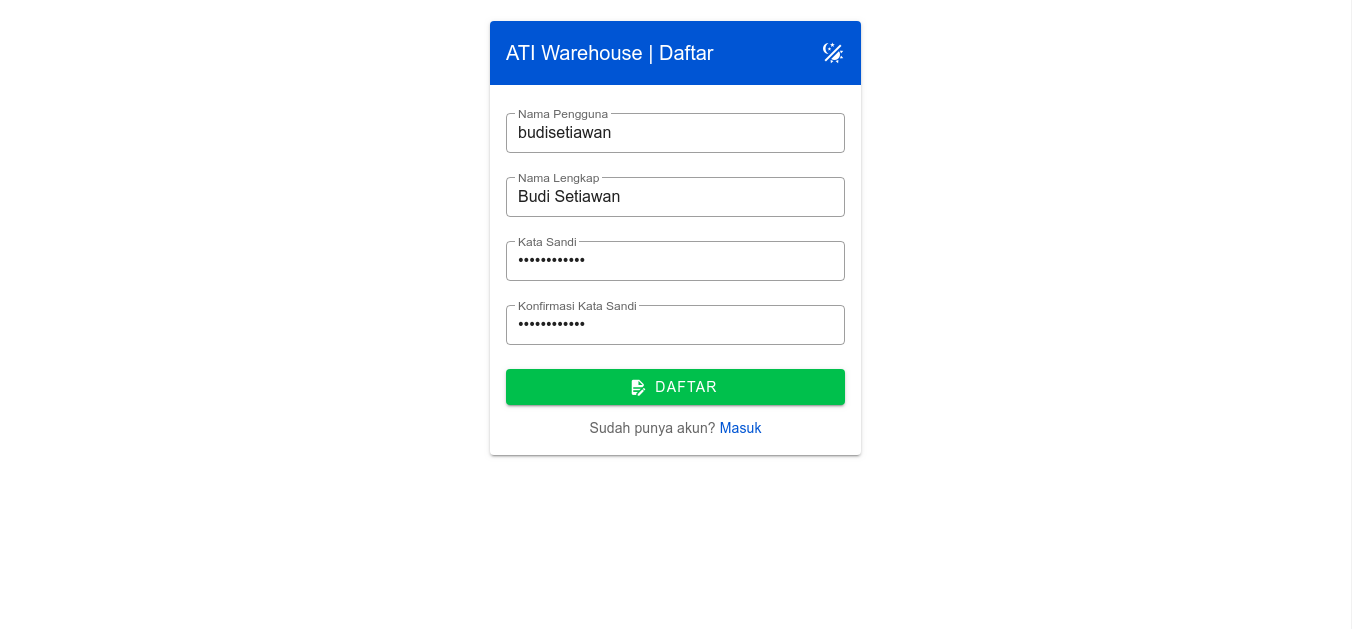
\includegraphics[width=0.95\textwidth]{gambar/mendaftar-akun.png}
  \caption{Tampilan Halaman Pendaftaran Akun Baru}
	\label{fig:mendaftarAkun}
\end{figure}

Pada sistem yang kami buat, sebelum bisa login, akun baru harus diverifikasi terlebih dahulu oleh admin untuk menghindari akses dari akun yang tidak diinginkan.
Verifikasi sendiri bisa dilakukan pada halaman daftar pengguna menggunakan akun admin seperti yang terlihat pada gambar \ref{fig:daftarPengguna}.
\vspace{0.5ex}

\begin{figure} [ht!] \centering
  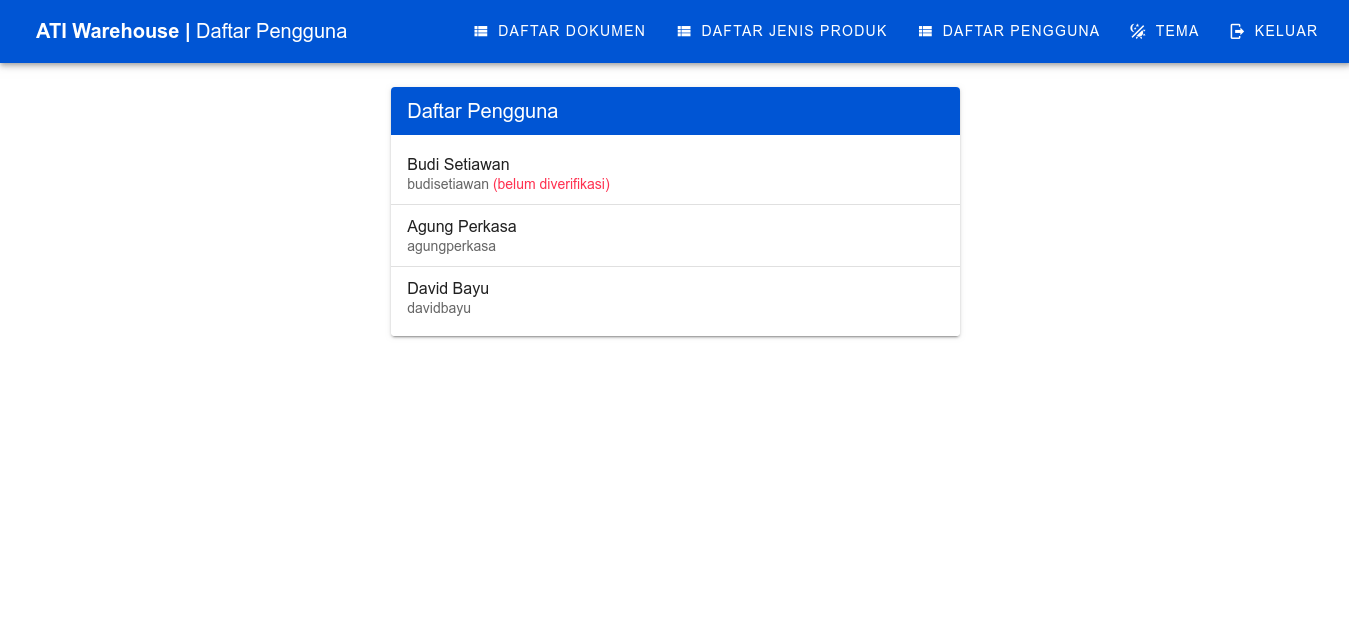
\includegraphics[width=0.95\textwidth]{gambar/daftar-pengguna.png}
  \caption{Tampilan Halaman Daftar Pengguna}
	\label{fig:daftarPengguna}
\end{figure}

Pengujian kemudian dilanjutkan dengan melakukan login menggunakan akun yang sudah diverifikasi sebelumnya seperti yang terlihat pada gambar \ref{fig:loginAkun}.
Setelah login berhasil, tampilan akan berpindah ke halaman utama yang berisi data dari keseluruhan administrasi loading barang.
\vspace{0.5ex}

\begin{figure} [ht!] \centering
  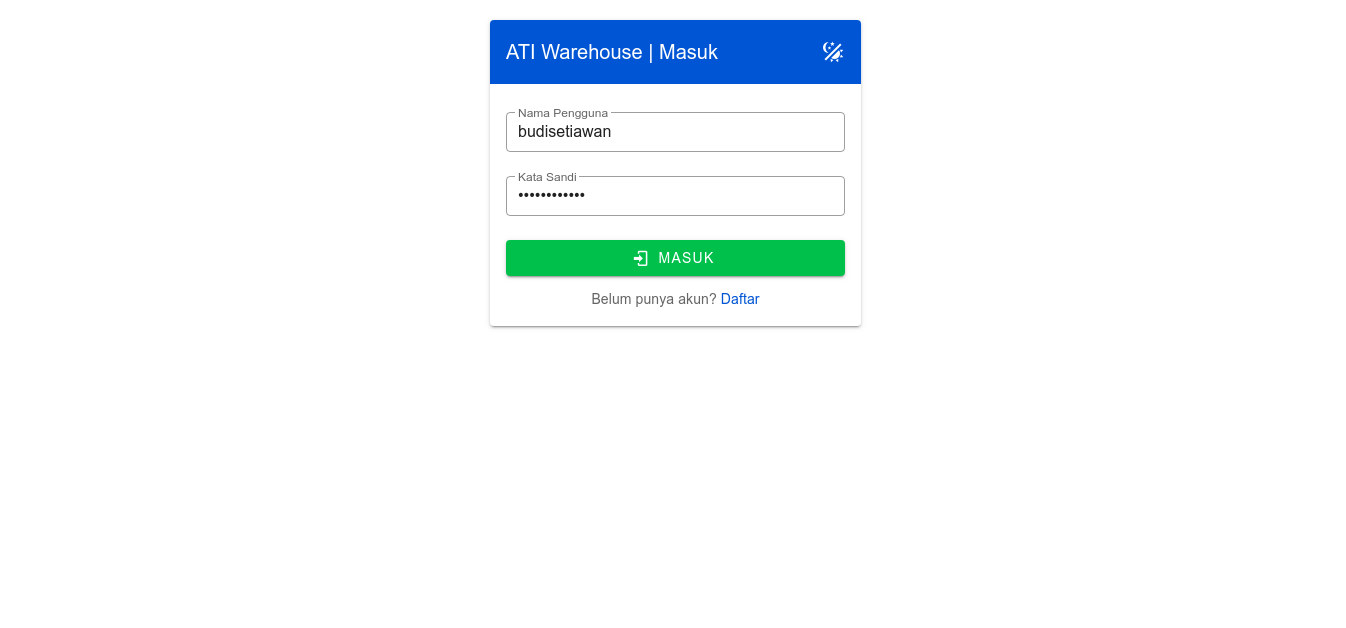
\includegraphics[width=0.95\textwidth]{gambar/login-akun.png}
  \caption{Tampilan Halaman Login Akun}
	\label{fig:loginAkun}
\end{figure}

Dari pengujian yang telah dilakukan tersebut dapat disimpulkan bahwa sistem yang telah kami buat bisa digunakan untuk melakukan login serta registrasi untuk pembuatan akun baru.
Dengan ini, nantinya pengguna yang membutuhkan akses terhadap data administrasi loading barang bisa membuat akun baru yang kemudian dapat diverifikasi oleh admin agar bisa mengakses data tersebut.
\vspace{0.5ex}

\subsection{Menguji Penambahan, Pengubahan, dan Penghapusan Data}
\vspace{1ex}

\lipsum[4]
\vspace{0.5ex}

\subsection{Menguji PWA Pada Perangkat Mobile}
\vspace{1ex}

\lipsum[4]
\vspace{0.5ex}

\subsection{Menguji Pengunduhan Data Dalam Bentuk \emph{Spreadsheet}}
\vspace{1ex}

\lipsum[4]
\vspace{0.5ex}